\chapter{Architectural Design}

\section{Overview}

At the highest level of abstraction, the architecture of Data4Help and AutomatedSOS system is a common three-tier client/server paradigm, as shown in Figure \ref{f:3tier}.





\begin{figure}[H]
\centering
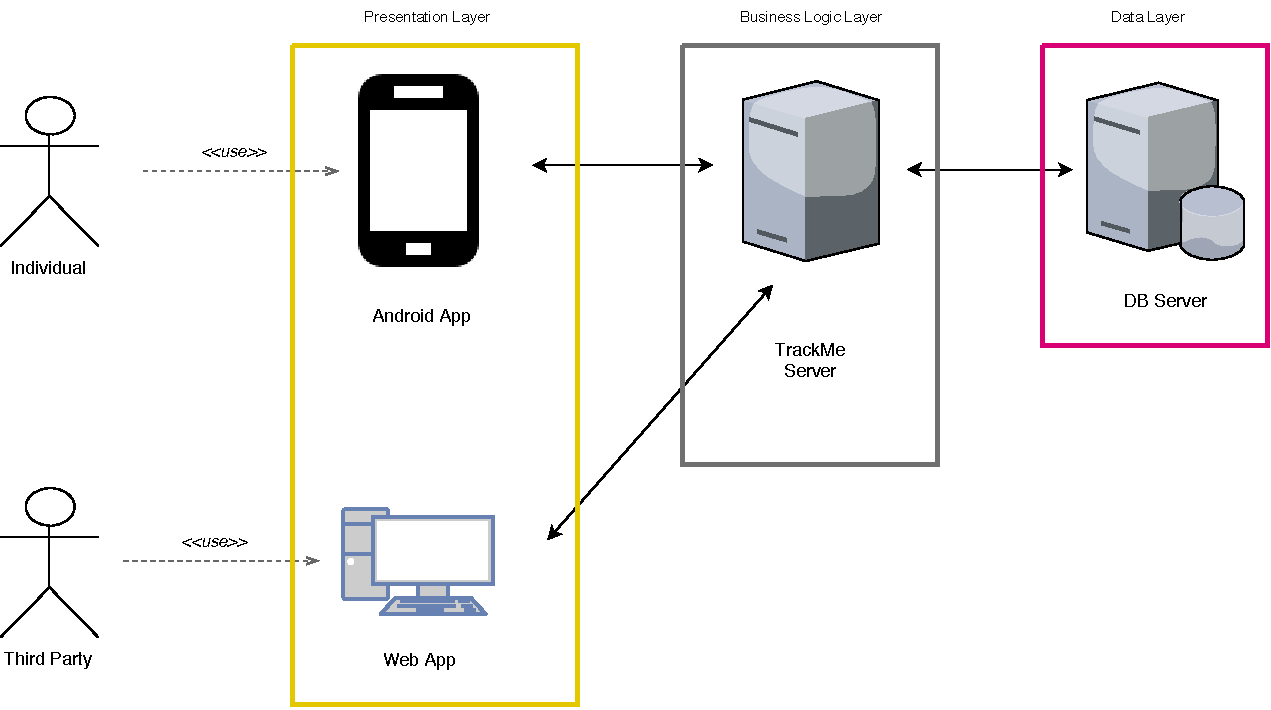
\includegraphics[scale=0.65]{resources/overview}
\caption{The 3 tier architecture of the system}\label{f:3tier}
\end{figure}
\noindent
The three layers are the following:

\begin{itemize}
\item \textbf{Presentation layer}: this layer is hosted on the users' devices, that are the smartphone for the individuals and a computer with a browser for third parties.
The GUIs are deployed in this layer.
\item \textbf{Business logic layer}: this layer contains the main components of the systems that carry out the operations needed for Data4Help and AutomatedSOS services.
\item \textbf{Data layer}: this layer is responsible for managing all the data of the system. 
In particular, it stores the data on persistent devices and makes them available when requested by the TrackMe servers.
\end{itemize}
The structure displayed in Figure \ref{f:3tier} is not to be understood as a rigid constraint on the implementation choices, but it represents where most of the three three logic layers are deployed.
For examples, it is possible that part of the data is (temporarily) stored on the clients in order to reduce latency or that some presentation logic is deployed on the TrackMe Server in order to achieve a more dynamic GUI.





\section{Component view}
The diagram in Figure \ref{f:comp_diag} examines in more detail the subcomponents composing the TrackMe server.
Some components requires external services, this is shown by means of pending required interfaces.
All the four components defined below have access to the database server interface in order to store and retrieve the data necessary for their correct operation.

\begin{figure}[H]
\centering
\includegraphics[width=\linewidth]{resources/uml/compdiag}
\caption{Component Diagram}\label{f:comp_diag}
\end{figure}

\noindent
As shown, there are four main components in the business logic server:

\begin{itemize}
\item \textit{Login Manager}: is responsible for the login and registration of the users, both individuals and third parties.
\item \textit{Data Collector}: is responsible of collecting data from the Android App. 
It also forwards the proper data to the Automated SOS component.

\item \textit{Data Manager}: receives and handles requests from third parties and push to them new data when available and the subscription is valid.
For certain functionalities, for example for geographically filter the data, the Data Manager component requires an external API to a map service.
It also makes possible for the individuals to visualize their data.

\item \textit{Automated SOS}: handles the subscriptions for the SOS service. 
Every time that it receives new data from the Data Collector, the component checks whether the thresholds are crossed, in this case it immediately calls an ambulance through an external API.
\end{itemize}
In addition, Figure \ref{f:comp_diag} shows that the Android App component requires an interface towards the wearable device, from which it will gather the eHealth Data.




\section{Deployment view}



The diagram in Figure \ref{f:depl_diag} shows the physical deployment of system's artifacts on various nodes.
In particular, the nodes are:

\begin{itemize}
\item \textit{Smartphone}: this device is used by an individual, then the Android Application is deployed here. This node interacts with the Business Server.
\item \textit{Personal Computer}: this device is used by a third party, only a modern browser compatible with HTML5 and CSS3 is required. Actually, there are no artifacts of our system deployed on this node, because the interaction is carried out with a Web App directly towards the Business Server.
\item \textit{Business Server}: this is the core node of our system.
All the Business Logic is deployed here, possibly by means of an Application Server like GlassFish.
This is the only node that interact with the Database node.
\item \textit{Data Server}: on this node are deployed all the artifacts necessary to manage the data.
\end{itemize}


\begin{figure}[h]
\centering
\includegraphics[width=\linewidth]{resources/uml/depldiag}
\caption{Deployment Diagram}\label{f:depl_diag}
\end{figure}



























